\chapter{Экспериментальная часть}
В этом разделе будет продемонстрирована работа программы, а также
приведены результаты замер времени работы реализаций алгоритмов.

\section{Демонстрация работы программы}
На рисунке 4.1, 4.2 приведена демонстрация работы программы.

\FloatBarrier
\begin{figure}[h!]
	\begin{center}
		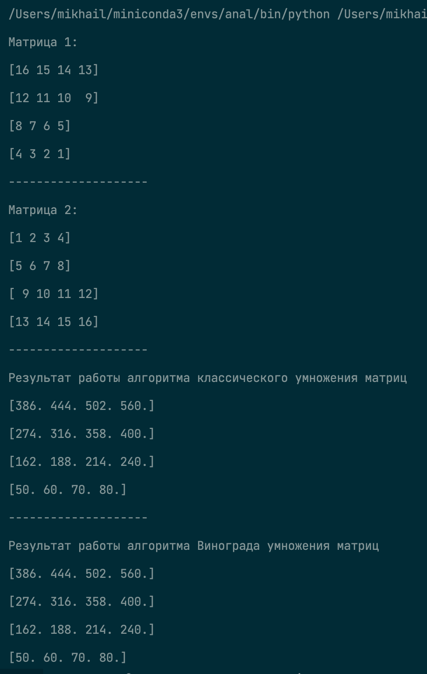
\includegraphics[width=80mm]{inc/demonstrate.png}
	\end{center}

	\caption{Демонстрация работы программы}
\end{figure}

\begin{figure}
	\begin{center}
	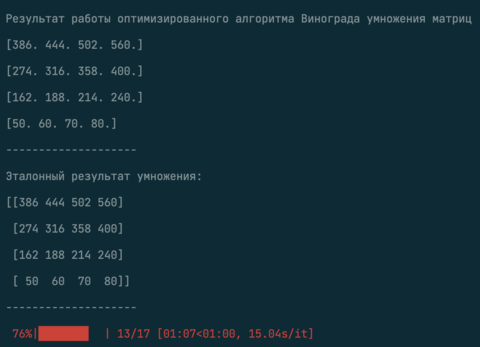
\includegraphics[]{inc/demonstrate_2.png}
	\end{center}
	\caption{Демонстрация работы программы (2 часть)}
\end{figure}
\FloatBarrier

\section{Технические характеристики}
Технические характеристики устройства, на котором выполнялось измерение времени, следующие:
\begin{itemize}
	\item операционная система: Mac OS 12.5.1;
	\item память: 8 Гб;
	\item процессор: Apple M2 3.5ГГц \cite{intel}.
\end{itemize}

\section{Измерение времени работы реализации алгоритмов}
Для определения быстродействия работы реализации алгоритмов будет проведено исследование зависимости
на квадратных матрицах, так как её размер однозначно определяется по одной переменной. 
По оси X будет откладываться размер квадратной матрицы, а по оси Y - время работы реализации алгоритмов
в наносекундах.

\subsection{Измерение времени работы реализации алгоритмов при чётном размере матрицы}
В таблице 4.1 представлены результаты замера времени работы реализации алгоритмов при чётном размере
квадратной матрицы.

\FloatBarrier
\begin{table}[h!]
	\centering
	\begin{center}
	\begin{threeparttable}
	\caption{Результаты замеров для чётных размеров матрицы}

	\begin{tabular}{ | l | l | l | l |}
		\hline
		Размер массива & Classic & Vinograd & optVinograd \\ \hline
		2 &       1252 &       1976 &          1816 \\
		4 &       4652 &       6302 &          6054 \\
		6 &      15088 &      16872 &         16860 \\
	   10 &      61236 &      58064 &         55992 \\
	   16 &     224896 &     210142 &        203270 \\
	   30 &    1449000 &    1281666 &       1263400 \\
	   50 &    6614733 &    5659400 &       5488600 \\
	   76 &   23076466 &   20108866 &      19752533 \\
	  100 &   53855066 &   44686000 &      44380266 \\
	  200 &  442294000 &  356596000 &     355450000 \\
	  400 & 3416924000 & 2861938000 &    2855959000 \\
		\hline
	\end{tabular}
\end{threeparttable}
\end{center}
\end{table}
\FloatBarrier

На рисунке 4.2 изображён график времени работы реализации алгоритмов от размера 
квадратной матрицы при чётных размерах матрицы.

\FloatBarrier
\begin{figure}[h!]
	\begin{center}
		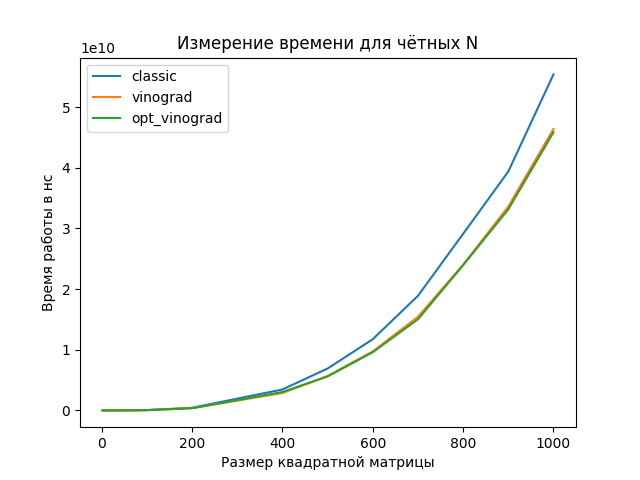
\includegraphics[width=\linewidth]{inc/chet.png}
	\end{center}
	\caption{График времени работы реализации алгоритмов умножения на матрицах чётных размеров}
\end{figure}
\FloatBarrier

\subsection{Измерение времени работы реализации алгоритмов при нечётном размере матрицы}
В таблице 4.2 представлены результаты замера времени работы реализации алгоритмов при нечётном размере
квадратной матрицы.

\FloatBarrier
\begin{table}[h!]

	\centering
	\begin{center}
	\begin{threeparttable}
	\caption{Результаты замеров для нечётных размеров матрицы}
	\begin{tabular}{ | l | l | l | l |}
		\hline
		Размер массива & Classic & Vinograd & optVinograd \\ \hline
		1 &        686 &       1062 &           970 \\
		3 &       2404 &       3506 &          3082 \\
		5 &       8104 &      10330 &          9280 \\
		9 &      41070 &      44068 &         42004 \\
	   15 &     185622 &     181722 &        172134 \\
	   31 &    1600666 &    1419933 &       1397066 \\
	   51 &    7070066 &    6048733 &       5884666 \\
	   75 &   21903200 &   18613733 &      18326133 \\
	  101 &   53137800 &   44933000 &      44198600 \\
	  201 &  431715000 &  353129000 &     367076000 \\
	  401 & 3399389000 & 2913350000 &    2841272000 \\
	\hline
	\end{tabular}
\end{threeparttable}
\end{center}
\end{table}
\FloatBarrier

На рисунке 4.3 изображён график времени работы алгоритмов от размера 
квадратной матрицы при нечётных размерах матрицы.

\FloatBarrier
\begin{figure}[h!]
	\begin{center}
		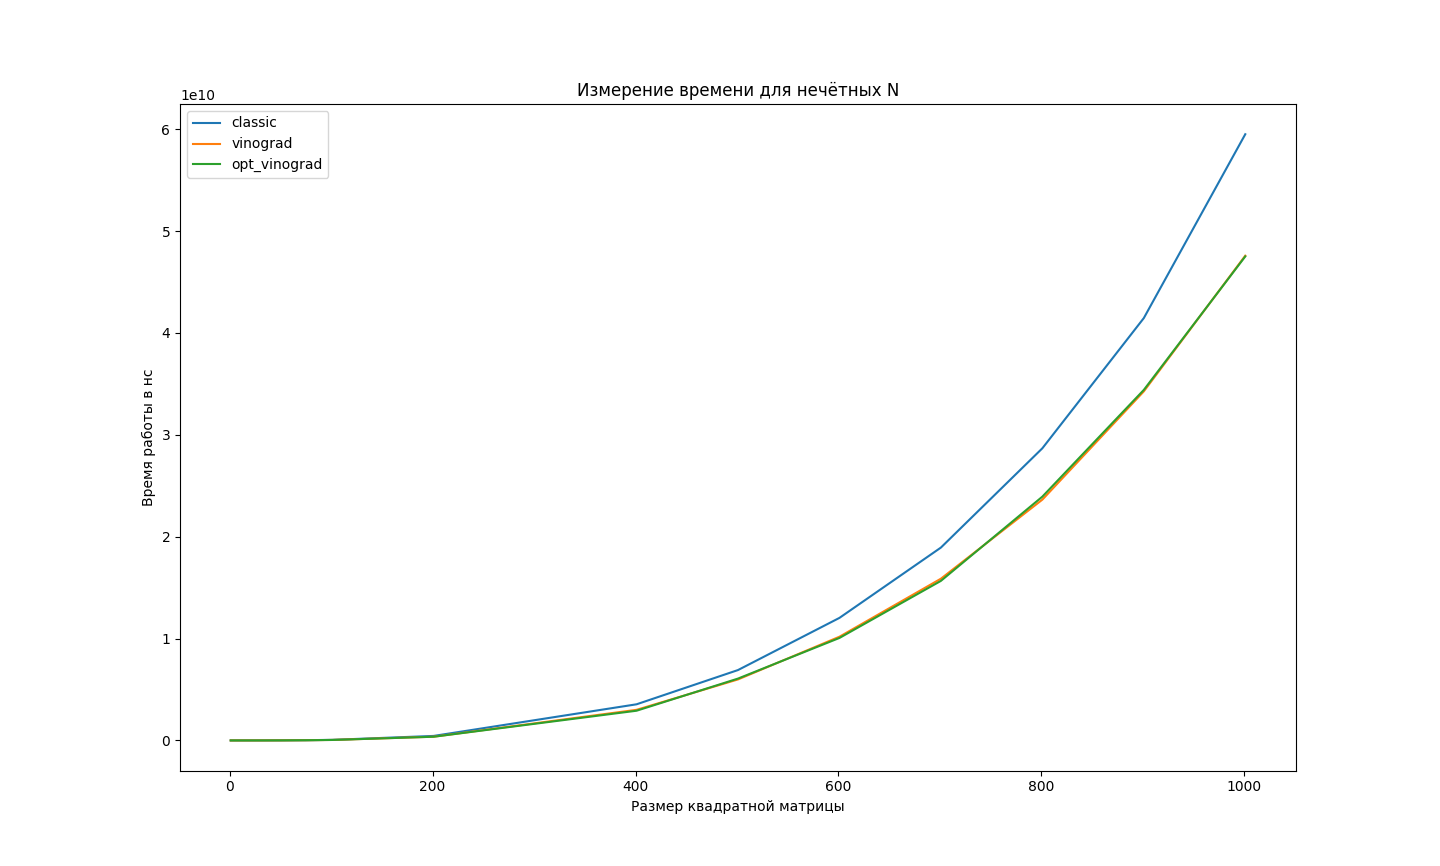
\includegraphics[width=\linewidth]{inc/nechet.png}
	\end{center}
	\caption{График времени работы алгоритмов умножения на матрицах нечётных размеров}
\end{figure}
\FloatBarrier

\section{Актуальность}

Если включить оптимизацию компилятора (для сравнения был выбран флаг O3), можно увидеть что алгоритм Винограда без ручной оптимизации выполняется быстрее.
Алгоритм умножения матриц Вионаграда по-прежнему выполняется быстрее классического.
Из сравнения можно сделать вывод, что ручная оптимизация алгоритмов не всегда оправданна, и часто компилятор знает лучше, как оптимизировать код.
Тем не менее, использование алгоритма с другой асимптотикой бывает оправданно.

\FloatBarrier
\begin{figure}[h!]
	\begin{center}
		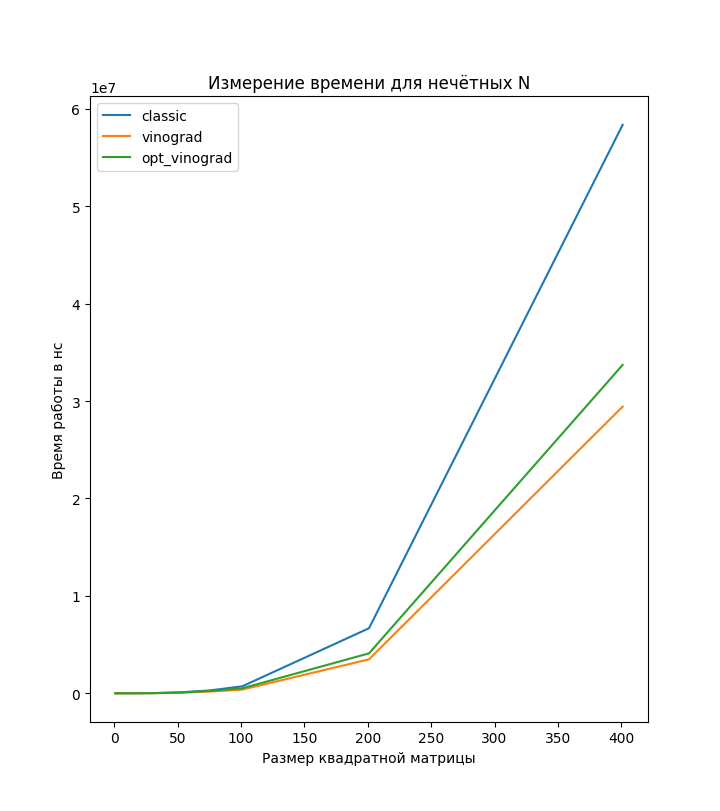
\includegraphics[width=\linewidth]{graph/optimized_comp.png}
	\end{center}
	\caption{График времени работы алгоритмов со включенной оптимизацией (-O3)}
\end{figure}
\FloatBarrier

\section*{Вывод}
Была написана программа, реализующая три алгоритма для умножения матриц.
Было проведено исследование зависимости работы алгоритмов от размера квадратной матрицы.

Удалось подтвердить, что у всех алгоритмов один и тот же порядок зависимости, 
что было предположением в секции оценке трудоёмкости работы.

Если размеры матрицы четные, обе реализации алгоритма Винограда работали быстрее классического алгоритма.
При размере $N=400$ оба алгоритма Винограда работают в два раза быстрее. При этом оптимизированный
алгоритм сработал на 18\% быстрее.

При нечетных размерах матрицы обе реализации алгоритма Винограла снова показали производительнось превосходящую классическую реализацию.
Полагая размер размере $N=401$ оптимизированный алгоритм Винограда работал на 2.5\%, чем обычный Виноград, 
и на 16\% -- чем классический алгоритм. Для $N=201$ аналогичные пропорции составили 
-4\% и 15\% соответственно.

Тем не мненее, при значения $N<6$ классический алгоритм работает быстрее, чем алгоритм Винограда,
и для матриц маленького размера подобные подсчеты и оптимизации не имеют смысл.

Рассматривая затраты памяти, классический алгоритм имеет зависимость $O(1)$, а алгоритмы Винограда -- $O(N)$.
Это связано с тем, что в алгоритмах Винограда значения сохраняются промежуточные в массивы. 
